%-------------------------------------------------------------------------------
%                            BAB IV
%               		HASIL DAN PEMBAHASAN
%-------------------------------------------------------------------------------
\fancyhf{}
\fancyfoot[C]{\thepage}
\chapter{HASIL DAN PEMBAHASAN}
\section{ANALISIS KEBUTUHAN}

Hasil dari analisis kebutuhan yang telah dilakukan adalah mendapatkan kelompok pengguna yang akan terlibat dalam penelitian dan \textit{use case diagram} untuk masing-masing pengguna. Berikut hasil analisis kebutuhan dari sistem yang dibangun.
\subsection{Kelompok Pengguna}
Kelompok pengguna dari aplikasi ini telah dapat diidentifikasikan pada tahap analisis kebutuhan pada sistem. terdapat 2 kelompok pengguna yang menggunakan aplikasi ini:
\begin{enumerate}[1.]
	\item Peneliti
	      \newline Pengguna yang menggunakan Aplikasi Mapping berbasis Android untuk melakukan pemetaan kekuatan sinyal atau nilai RSSI dari Beacon.
	\item Pengguna gedung FMIPA USK
	      \newline Pengguna yang menggunakan Aplikasi Penentuan Lokasi dan Estimasi Orang di gedung Fakultas Matematika dan Ilmu Pengetahuan Alam Univesitas Syiah Kuala berbasis Android.
\end{enumerate}

\subsection{Use Case Diagram}
\textit{Use case} diagram adalah diagram yang mendeskripsilam hubungan antara aktor dan sistem. \textit{Use case} diagram bisa mendeskripsikan sebuah interaksi antara satu atau lebih aktor dengan sistem yang akan dibuat. \textit{Use case} diagram juga bisa digunakan untuk mengetahui fungsi apa saja yang ada di dalam sebuah sistem dan  bisa juga mempresentasikan sebuah interaksi aktor dengan sistem. Komponen tersebut kemudian menjelaskan komunikasi antara aktor,  dengan sistem yang ada. Dengan demikian, \textit{use case} dapat dipresentasikan dengan urutan yang sederhana, dan akan mudah dipahami oleh para konsumen \citep{Yu2009}. \textit{Use Case Diagram} dari sistem yang telah dibangun dapat dilihat pada Gambar \ref{usecasemapping} dan Gambar \ref{usecasedosen}

\begin{figure}[H]
	\center
	\shadowbox
	{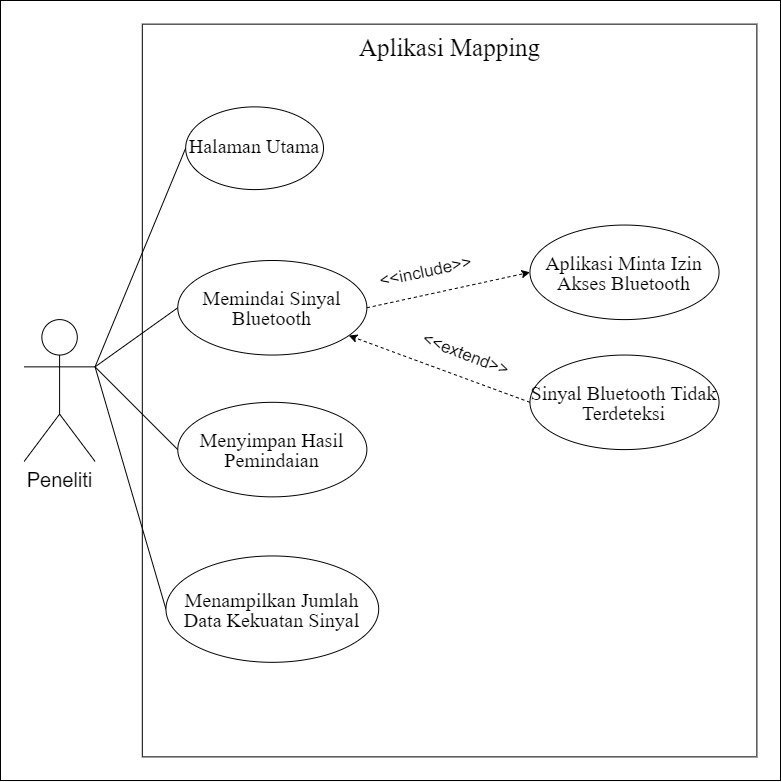
\includegraphics [width=8.5cm, height=8cm]{gambar/mapping}}
	\caption{\textit{Use Case Diagram} Aplikasi Mapping.}
	\label{usecasemapping}
\end{figure}

\par Gambar \ref{usecasemapping} diatas menjelaskan aktivitas yang dapat dilakukan oleh peneliti saat menggunakan aplikasi mapping. Ketika peneliti membuka aplikasi mapping, maka akan muncul halaman beranda. Kemudian, peneliti diminta untuk mengizinkan aplikasi mengakses lokasi pada perangkat. Selanjutnya, peneliti dapat melakukan pemindaian kekuatan sinyal setelah menghidupkan Bluetooth pada perangkat \textit{smartphone}. Setelah itu, hasil dari pemindaian kekuatan sinyal tersebut disimpan didalam server dan dapat ditampilkan jumlah data kekuatan sinyal.
\fancyhf{}
\fancyfoot[R]{\thepage}
\begin{figure}[H]
	\center
	\shadowbox
	{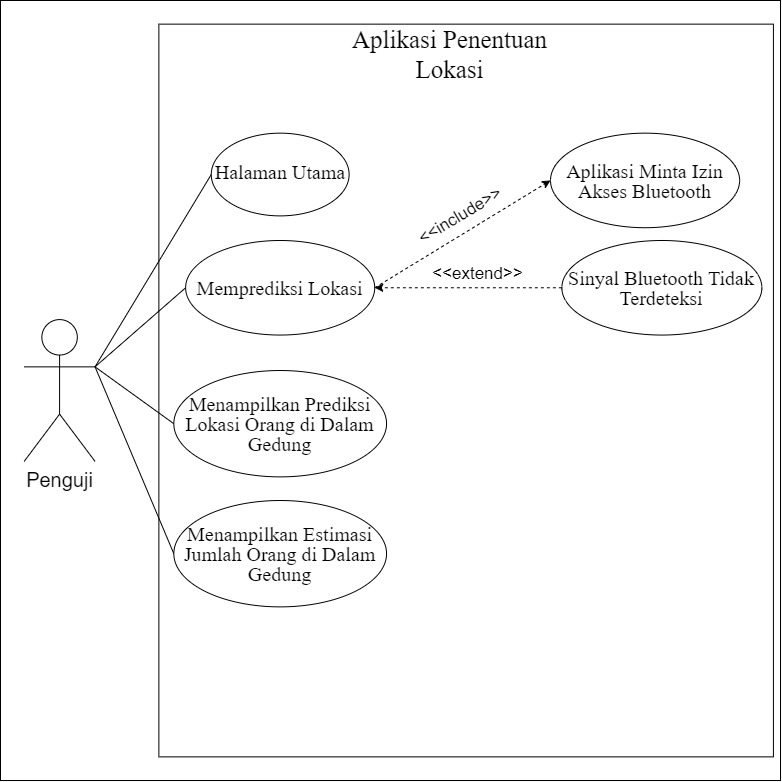
\includegraphics [width=10cm, height=9cm]{gambar/penentuanlokasi}}
	\caption{\textit{Use Case Diagram} Aplikasi Penentuan Lokasi dan Estimasi Orang}
	\label{usecasedosen}
\end{figure}

\par Gambar \ref{usecasedosen} menjelaskan aktivitas yang dapat dilakukan oleh setiap orang yang memasuki gedung Fakultas Matematika dan Ilmu Pengetahuan Alam Universitas Syiah Kuala. Aktivitas pertama yang dapat dilakukan adalah membuka aplikasi LocaLization, pengguna dapat menikmati fitur-fitur yang tersedia seperti melihat estimasi atau jumlah orang yang sedang berada didalam gedung, memulai proses pengecekan lokasi diri sendiri saat berada didalam gedung FMIPA USK dengan syarat keadaan \textit{Bluetooth} pada perangkat dalam keadaan hidup dan melihat kecepatan prediksi berapa detik. Jika pengguna berada diluar gedung FMIPA USK, maka perangkat akan memprediksi pengguna sedang berada diluar jangkauan.


% //TODO:Selanjutnya Buat diagram Deployment
\section{PERANCANGAN DAN PEMBUATAN SISTEM}

\subsection{Perancangan Sistem}
\par Perancangan sistem merupakan tahapan proses desain dari sistem perangkat lunak yang dibuat. Proses ini terdiri dari dua tahap yaitu perancangan konfigurasi eksekusi sistem dalam bentuk \textit{deployment diagram} dan perancangan tampilan antar muka (\textit{interface}).

Tahap pertama adalah merancang \textit{deployment diagram}, dimana \textit{deployment diagram} adalah diagram yang menjelaskan bagaimana sistem bekerja dan digunakan oleh pengguna. Berikut rancangan \textit{deployment diagram} dari sistem yang telah dibangun dapat dilihat pada Gambar \ref{deployment-diagram}.

%\begin{enumerate}
%\item \textit{Deployment Diagram} Aplikasi Mapping
\vspace{-0.2cm}
\begin{landscape}
	\begin{figure}[H]
		\center
		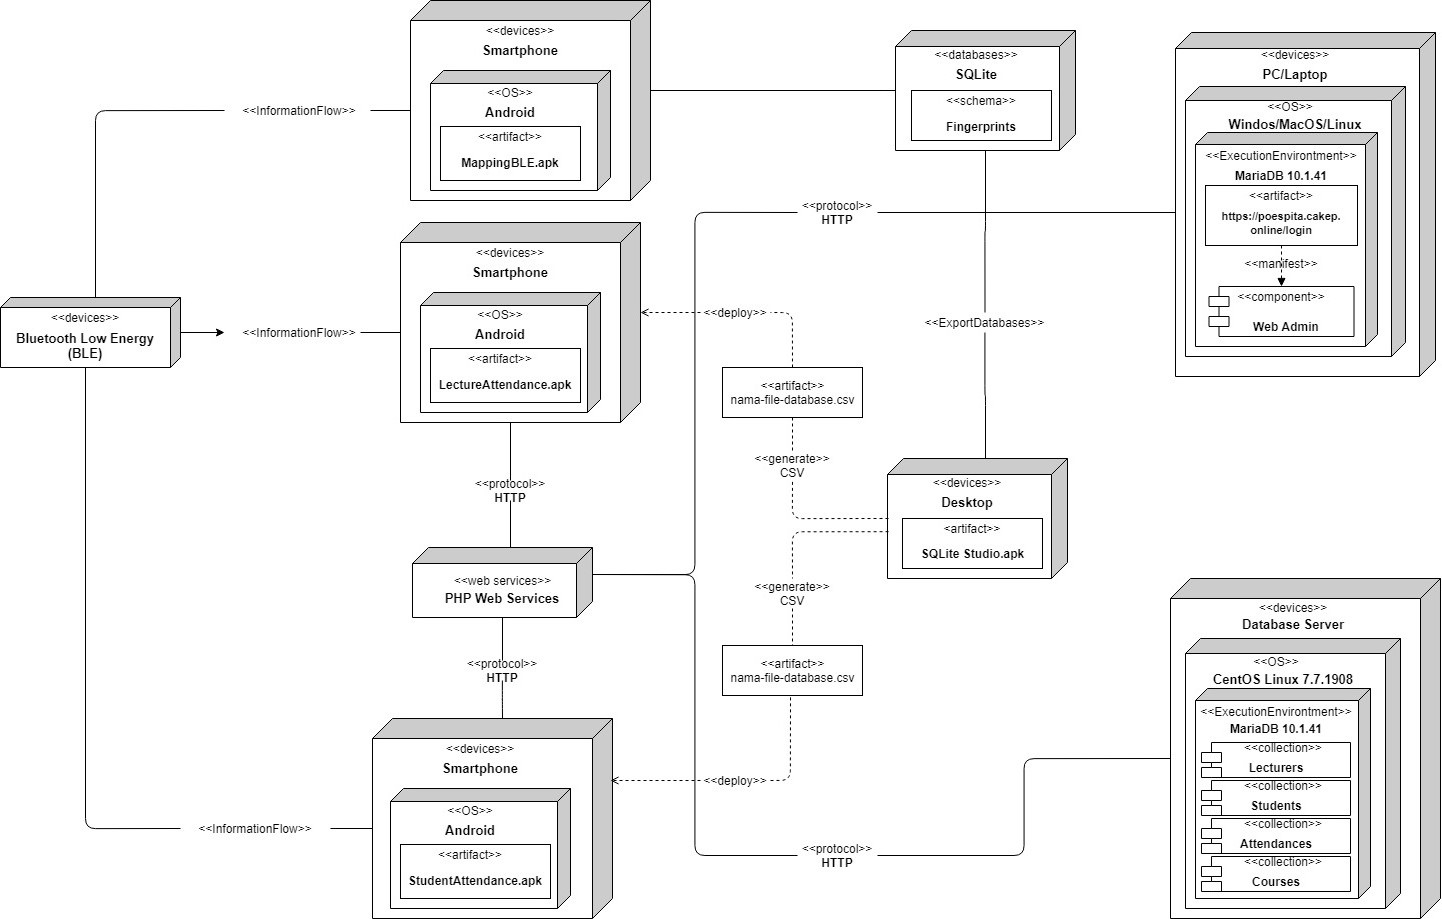
\includegraphics [width = 22.5cm, height=12cm]{gambar/model/deployment-diagram}
		\caption{Diagram \textit{Deployment}}
		\label{deployment-diagram}
	\end{figure}
\end{landscape}

Tahap kedua adalah merancang tampilan antar muka pengguna (\textit{user interface}) sebagai mekanisme komunikasi dengan sistem. Antar muka dari sistem yang telah dibangun adalah sebagai berikut:
\begin{enumerate}[a.]

	\item Antar Muka Aplikasi Mapping
	      \par Gambar \ref{aplikasimappingbagian1} menampilkan halaman awal ketika aplikasi pertama dibuka, pada halaman ini terdapat fitur untuk memasukkan nama tempat, serta fitur untuk menampilkan informasi   nama \textit{device} Bluetooth, RSSI, dan \textit{MAC address} Bluetooth, Serta pada bagian bawah terdapat empat fitur  yang masing-masing memiliki  fungsi untuk memindai , menampilkan waktu tunggu, menyimpan data dan menampilkan jumlah data yang telah disimpan. Apabila pengguna melakukan pemindaian maka akan muncul notifikasi untuk mengaktifkan Bluetooth. Apabila Bluetooth sudah hidup, maka aplikasi akan mencari nama \textit{device} Bluetooth, RSSI dan dan \textit{MAC address} Bluetooth yang ada di sekitar, pada bagian bawah fitur pemindai akan berubah menjadi stop dan fitur waktu akan menampilkan waktu tunggu  selama 10 detik, waktu ini digunakan  untuk menyamaratakan waktu pemindaian untuk setiap data. Kemudian setelah data disimpan, pada fitur yang menampilkan jumlah data yang telah disimpan yang awalnya 0 sekarang menjadi 1 yang berarti 1 data sudah dimasukkan ke dalam \textit{database server}.

	      \vspace{-0cm}
	      \begin{figure} [H]
		      \begin{subfigure}{.5\textwidth}
			      \centering
			      % include first image
			      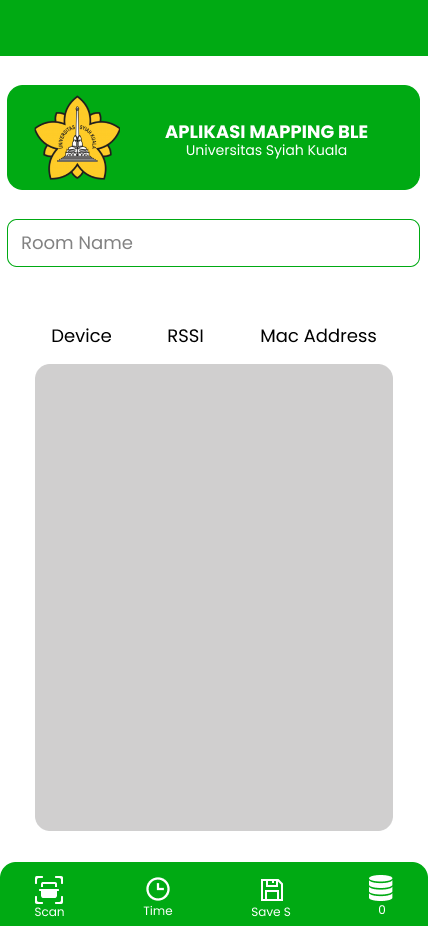
\includegraphics[width=.5\linewidth]{gambar/mapping1.png}
			      \caption{Halaman awal aplikasi \textit{mapping}}
		      \end{subfigure}
		      \begin{subfigure}{.5\textwidth}
			      \centering
			      % include second image
			      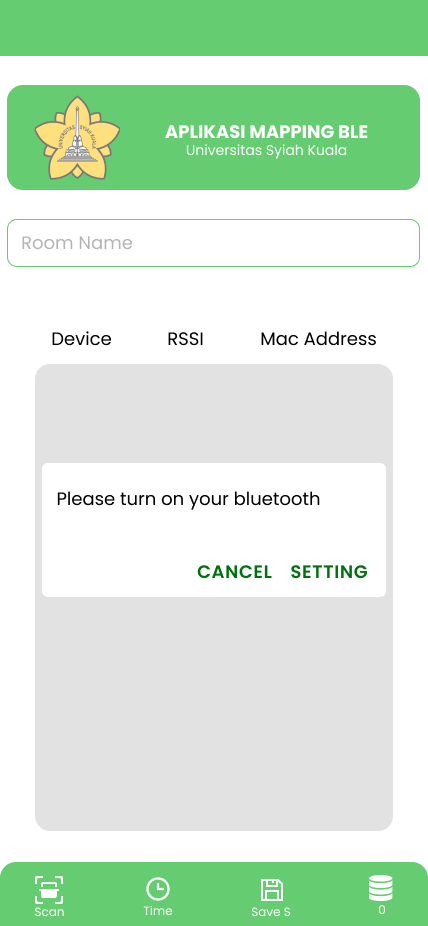
\includegraphics[width=.5\linewidth]{gambar/mapping2.png}
			      \caption{Izin mengakses Bluetooth}
		      \end{subfigure}
		      \vspace{1cm}
		      \newline
		      \begin{subfigure}{.5\textwidth}
			      \centering
			      % include third image
			      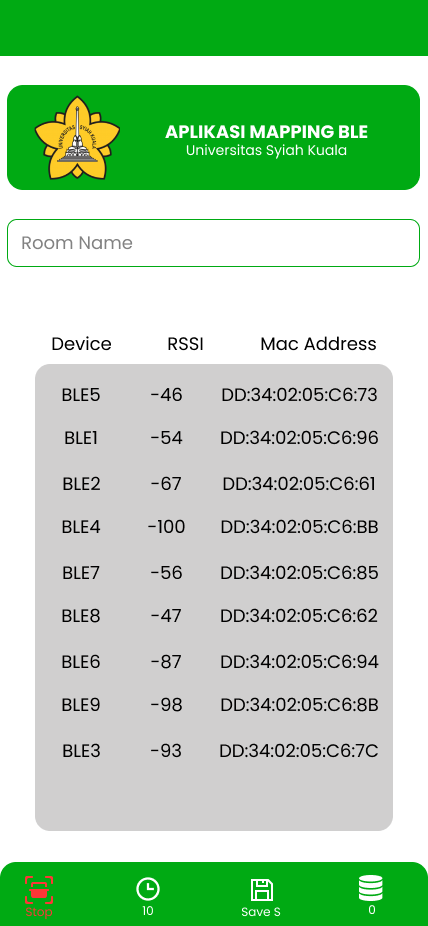
\includegraphics[width=.5\linewidth]{gambar/mapping3.png}
			      \caption{Proses pemindaian kekuatan sinyal}
		      \end{subfigure}
		      \begin{subfigure}{.5\textwidth}
			      \centering
			      % include fourth image
			      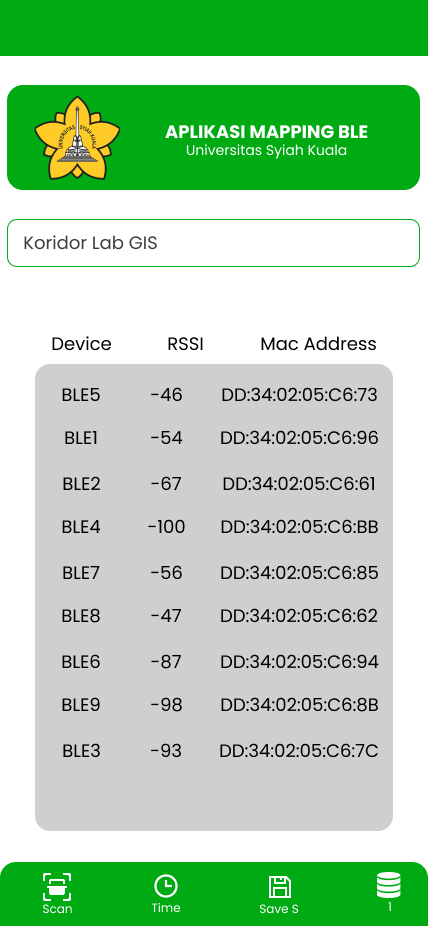
\includegraphics[width=.5\linewidth]{gambar/mapping4.png}
			      \caption{Selesai proses pemindaian}
		      \end{subfigure}
		      \vspace{0.5cm}
		      \caption{Tampilan Halaman Aplikasi Mapping}
		      \label{aplikasimappingbagian1}
	      \end{figure}

	      \vspace{1cm}
	\item Antar Muka Aplikasi SpecifyLocation

	      \par Gambar \ref*{aplikasiPenentuanLokasi} memperlihatkan ketika pengguna berada di halaman utama dari aplikasi SpecifyLocation, dimana akan terlihat beberapa informasi dan fitur yang dimiliki oleh aplikasi SpecifyLocation seperti estimasi jumlah orang yang berada di dalam gedung FMIPA USK, kecepatan prediksi, lokasi hasil prediksi dan algoritma yang digunakan serta satu tombol cek lokasi untuk melakukan pencarian lokasi pengguna. Ketika pengguna menekan tombol cek lokasi, maka aplikasi akan menampilkan notifikasi untuk menghidupkan Bluetooth jika Bluetooth pada perangkat yang digunakan belum hidup. Jika Bluetooth sudah hidup di perangkat yang digunakan maka aplikasi akan memprediksi lokasi pengguna saat ini, jika pengguna sedang berada di luar gedung A FMIPA USK, maka akan tampilan aplikasi tidak akan beruah, namun jika pengguna berada di dalam gedung A FMIPA USK maka aplikasi akan memeprediksi lokasi pengguna yang dapat dilihat dengan adanya denah gedung A FMIPA USK serta lokasi hasil prediksi akan berubah warna.

	      \vspace{-0cm}
	      \begin{figure} [H]
		      \begin{subfigure}{.5\textwidth}
			      \centering
			      % include first image
			      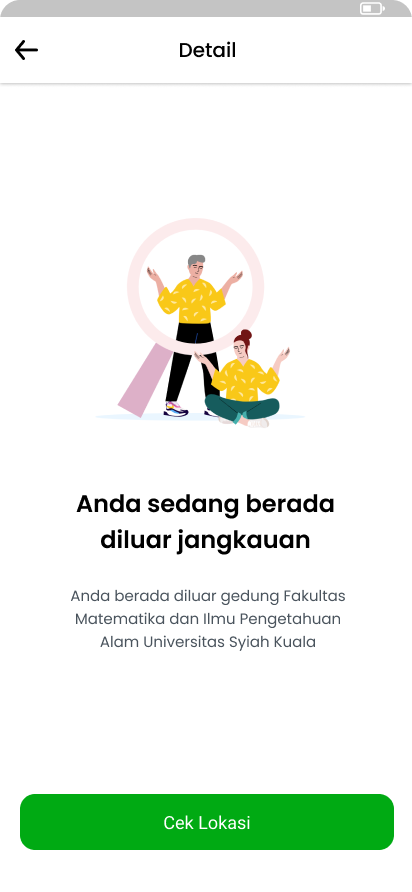
\includegraphics[width=.5\linewidth]{gambar/diluarjangkauan.png}
			      \caption{Halaman Awal dan Luar Gedung A FMIPA}
		      \end{subfigure}
		      \begin{subfigure}{.5\textwidth}
			      \centering
			      % include second image
			      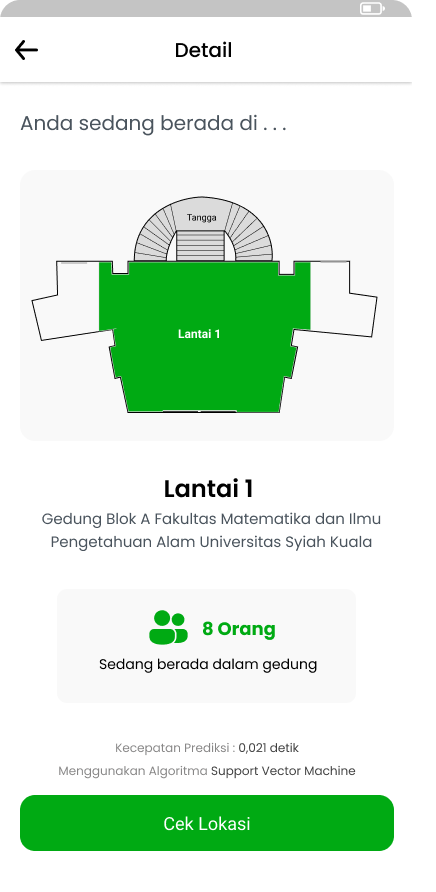
\includegraphics[width=.5\linewidth]{gambar/applantai1.png}
			      \caption{Hasil Prediksi Lantai 1}
		      \end{subfigure}
		      \vspace{1cm}
		      \newline
		      \begin{center}
			      \begin{subfigure}{.5\textwidth}
				      \centering
				      % include third image
				      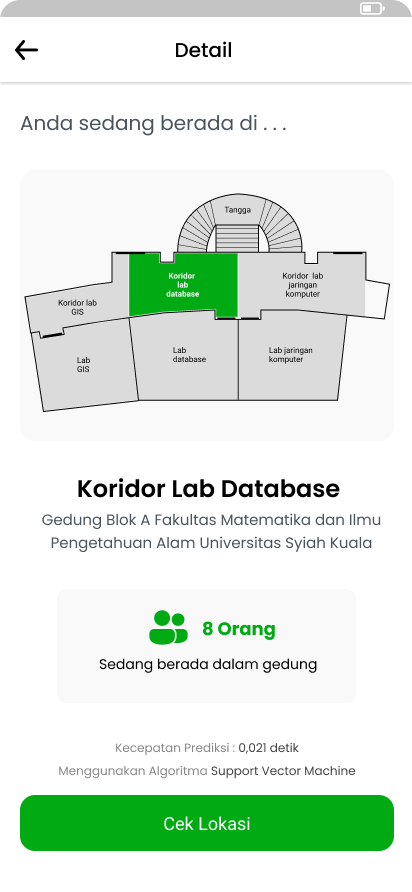
\includegraphics[width=.5\linewidth]{gambar/applantai3}
				      \caption{Hasil Prediksi Koridor Lab Data Base}
			      \end{subfigure}
		      \end{center}
		      \vspace{0.5cm}
		      \caption{Tampilan Halaman Aplikasi Penentuan Lokasi}
		      \label{aplikasiPenentuanLokasi}
	      \end{figure}

	      \vspace{0.5cm}

\end{enumerate}

%%%%%%%%%%%%%%%%%%%%%%%%%%%%%%%%%%%%%%%%%%%akhir perancangan aplikasi mapping%%%%%%%%%%%%%%%%%%%%%%%%%%%%%%%%%%%%%%%%%%%%%%%%%%%
\subsection{Pembuatan Sistem}

\begin{enumerate}[a.]
	\item Aplikasi \textit{Mapping}
	      \\ Aplikasi \textit{mapping} merupakan  aplikasi \textit{mobile} berbasis Android yang dibuat menggunakan bahasa pemrograman JavaScript dengan \textit{framework} React Native. Media untuk penyimpanan data pada aplikasi \textit{mapping} ini menggunakan \textit{database} MongoDb Compass yang datanya akan dikirim melalui \textit{Web Service}. Potongan kode program yang terdapat dalam aplikasi \textit{mapping} ini dapat dilihat pada Progran 4.1 berikut ini.
	      \vspace{0.4cm}
	      \lstset{language=Java,
		      basicstyle=\ttfamily\scriptsize\color{black},
		      keywordstyle=\color{javapurple}\bfseries,
		      stringstyle=\color{javared},
		      commentstyle=\color{javagreen},
		      morecomment=[s][\color{javadocblue}]{/**}{*/},
		      numbers=left,
		      numberstyle=\tiny\color{black},
		      showstringspaces=false,
		      numbersep=10pt,
		      tabsize=4,
		      showspaces=false,
		      showstringspaces=false,
		      autogobble=true,
		      xleftmargin=2em
	      }
	      \begin{lstlisting}[label=programScanBle]
			import React, { useState } from 'react';
			import {
				Image,StyleSheet,Text,FlatList,View,TouchableOpacity,Alert,
			} from 'react-native';
			import { ScrollView, TextInput } from 'react-native-gesture-handler';
			import { manager } from '../Ble';
			import AkunSvg from './../svg/AkunSvg';
			import { colors, sizes } from '../constants';
			import Card from '../components/Card';
			import Table from './../components/Table';
			import BottomNav from '../components/BottomNav';
			
			const HomeScreen = () => {
			  const [showData, setShowData] = useState<any[]>([]);
			  const [label, setLabel] = useState<string>('');
			  const handleDevices = (devices: any) => {
				setShowData(devices);
			  };
			  const renderItem = ({ item, index }: any) => (
				<View style={styles.dataTable} key={index}>
				  <Text style={[{ width: '40%' }]}>{item.name}</Text>
				  <Text style={[{ width: '20%' }]}>{item.rssi}</Text>
				  <Text style={[{ width: '40%' }]}>{item.macAddress}</Text>
				</View>
			  );
			  return (
				<View style={styles.container}>
				  <View style={styles.header}>
					<Text></Text>
				  </View>
			
				  <Card />
			
				  <View>
					<TextInput
					  style={styles.formInput}
					  placeholder={'Room Name'}
					  onChangeText={(value) => setLabel(value)}
					  value={label}
					/>
				  </View>
			
				  <View style={styles.tableContainer}>
					<View style={styles.headerTable}>
					  <Text style={[{ width: '40%' }]}>Devices</Text>
					  <Text style={[{ width: '20%' }]}>RSSI</Text>
					  <Text style={[{ width: '40%' }]}>Mac Address</Text>
					</View>
			
					{showData.length === 0 ? (
					  <ScrollView style={styles.listContainer}></ScrollView>
					) : (
					  <ScrollView style={styles.listContainer}>
						{showData.map((item, index) => {
						  return renderItem({ item, index });
						})}
					  </ScrollView>
					)}
				  </View>
			
				  <BottomNav onSetData={handleDevices} label={label} />
				</View>
			  );
			};
			
			export default HomeScreen;
	\end{lstlisting}
	      \captionof{lstlisting}{Potongan Kode Program dalam aplikasi \textit{mapping}.}


	\item Aplikasi SpecifyLocation
	      \\ Aplikasi SpecifyLocation adalah aplikasi \textit{mobile} berbasis Android yang dibuat menggunakan bahasa pemrograman JavaScript dan \textit{framework} React Native. Aplikasi ini akan memindai sinyal RSSI yang ada di dekat pengguna berada selama 10 detik, kemudian data sinyal RSSI tersebut akan di kirim ke API [Isi nanti] yang di dalamnya terdapat model yang sudah dibuat sebelumnya dengan menggunakan algoritma \textit{KMeans}. Kemudian API akan mengirimkan hasil prediksi lokasi saat ini dari model ke aplikasi SpecifyLocation, setelah itu aplikasi akan menampilkan hasil prediksinya serta beberapa informasi lainnya seperti kecepatan prediksi dan algoritma yang digunakan, jika pengguna berada di luar gedung A FMIPA USK fitur estimasi jumlah orang tidak akan bertambah, namun jika pengguna berada di dalam gedung A FMIPA USK maka fitur estimasi jumlah orang akan bertambah 1 dan jika pengguna menekan tombol cek lokasi kembali dan hasil prediksinya tetap di dalam gedung A FMIPA USK fitur estimasi jumlah orang tidak akan bertambah lagi, namun jika kemudian pengguna menekan tombol cek lokasi kembali setelahnya dan aplikasi memprediksi pengguna berada di luar gedung A FMIPA USK maka fitur estimasi jumlah orang akan berkurang 1. Potongan kode program yang terdapat dalam aplikasi ini dapat dilihat
	      pada Progran 4.2 berikut ini.

	      \vspace{0.4cm}
	      \begin{lstlisting}[label=programKNNDosen]
						import axios from "axios";
						import React, { useEffect, useState } from "react";
						import {
						  ScrollView,StyleSheet,Text,TouchableOpacity,View,Image
						} from "react-native";
						import Card from "../components/Card";
						import { colors, SCAN_PERIOD, sizes } from "../constants";
						import { blePermission, initBleScanner, startScan } from "../permission/Ble";
						import {
						  selectStatus,setEstimasiStatus,
						} from "../redux/features/location/locationSlice";
						import { useAppDispatch, useAppSelector } from "../redux/hooks";
						import GambarOrang from "../svg/GambarOrang";
						import GelombangAtas from "../svg/GelombangAtas";
						import GelombangBawah from "../svg/GelombangBawah";
						import HalamanAwal from "../svg/GelombangBawah";
						import GambarJumlahOrang from "../svg/JumlahOrang";
						import Lantai1 from "../svg/Lantai1";
						import Lantai3 from "../svg/Lantai3";
						import speed from "../svg/Kecepatan";
						import Kecepatan from "../svg/Kecepatan";
						import IconLokasi from "../svg/IconLokasi";
						import Algo from "../svg/Algo";
						interface BleDevice {
						  macAddress: string;
						  rssi: number;
						  name: string;
						}
						const HomeScreen = () => {
						  const [intervals, setIntervals] = React.useState(2);
						  const [cinterval, setcInterval] = React.useState(1);
						  const [width, setWidth] = React.useState(0);
						  const init = (width: number) => {
							// initialise width
							setWidth(width);
							// initialise total intervals
							const totalItems = 2;
							setIntervals(Math.ceil(totalItems / 1));
						  }
						  let bullets = [];
						  for (let i = 1; i <= intervals; i++) {
							bullets.push(
							  <Text
								key={i}
								style={{
								  ...styles.bullet,
								  opacity: cinterval=== i ? 1 : 0.5,
								}}
							  >
							  </Text>
							);
						  }
						  const getcInterval = (offset: any) => {
							for (let i = 1; i <= intervals; i++) {
							  if (offset < (width / intervals) * i) {
								return i;
							  }
							  if (i == intervals) {
								return i;
							  }
							}
						  }
						
						  const statusNow: string = useAppSelector(selectStatus);
						  const [lokasi, setLokasi] = useState<string>("");
						  const [waktu, setWaktu] = useState<number>(0);
						  const [estimasi, setEstimasi] = useState<number>(0);
						  const [deviceDefaults, setDeviceDefaults] = useState<BleDevice[]>([]);
						  const [textBtn, setTextBtn] = useState<string>("Cek Lokasi");
						  const [loading, setLoading] = useState<boolean>(false);
						  const [deviceTestings, setDeviceTestings] = useState<BleDevice[]>([]);
						  const dispatch = useAppDispatch();
						  // Interval Waktu
						  const setIntervalX = (
							callback: () => void,
							delay: number,
							repetitions: number
						  ) => {
							let x = 0;
							let intervalID = setInterval(function () {
							  callback();
						
							  if (++x === repetitions) {
								clearInterval(intervalID);
								setTextBtn("Cek Lokasi");
							  }
							}, delay);
						  };
						
						  // Prediksi
						  useEffect(() => {
							// prediksiData();
							let formdata = new FormData();
							formdata.append("algoritma", "kmeans");
							setInterval(() => {
							  axios
								.post(`https://api-model-flasks.herokuapp.com/api/estimasi`, formdata)
								.then((response) => {
								  setEstimasi(response.data.estimasi);
								})
								.catch((err) => console.log(err));
							}, 1000);
						
							initBleScanner().then((data: BleDevice[] | undefined) => {
							  if (data) {
								setDeviceDefaults(data);
								setDeviceTestings(data);
							  }
							});
						  }, []);
						
						  // Tombol
						  const handlePressBtn = () => {
							blePermission();
							setLoading(true);
							let detik = SCAN_PERIOD / 1000;
						
							setTextBtn(`Tunggu ${detik--} detik`);
							setIntervalX(
							  () => {
								setTextBtn(`Tunggu ${detik--} detik`);
							  },
							  1000,
							  detik
							);
							setDeviceTestings(deviceDefaults);
							// Scan
							startScan(deviceDefaults, deviceTestings, "kmeans", SCAN_PERIOD)
							  .then((data: any) => {
								setLoading(false);
								console.log(data);
								setLokasi(data.label);
								setWaktu(data.runtime);
								console.log(data.label);
								if (data.label === "Luar Gedung MIPA") {
								  return dispatch(setEstimasiStatus("keluar"));
								}
								return dispatch(setEstimasiStatus("masuk"));
							  })
							  .catch((err) => {
								setLoading(false);
								console.log(err);
							  });
						  };
    
    \end{lstlisting}
	      \captionof{lstlisting}{Potongan Kode Program dalam aplikasi SpecifyLocation.}

\end{enumerate}

\section{PENGUJIAN SISTEM}
\par Pengujian sistem dilakukan untuk melihat apakah sistem dapat berjalan dengan tepat sesuai dengan rancangan. Beberapa pengujian yang dilakukan pada penelitian ini adalah pengujian keakuratan prediksi dengan menggunakan algoritma \textit{kmeans}, pengujian usabilitas dengan metode UMUX dan pengujian fungsionalitas menggunakan \textit{Blackbox}.

\subsection{Pengujian Keakuratan Prediksi Menggunakan Algoritma \textit{Kmeans}}
\begin{enumerate}

	\item Pengujian Keakuratan Klasifikasi Reference Point

	      \par Pengujian ini dianalisis menggunakan metode klasifikasi K-NN. Pengujian ini bertujuan untuk menganalisis jenis penyebaran \textit{reference point} yang terbaik dengan membandingkan \textit{F-Measure} yang didapatkan dari setiap pengujian. Data \textit{training} yang digunakan pada penelitian ini sebanyak 764 data kekuatan sinyal dengan masing-masing 324 data kekuatan sinyal untuk \textit{reference point} acak, 440 data kekuatan sinyal untuk \textit{reference point} urut dan 160 sebagai data uji. Pengumpulan data \textit{training} dilakukan dengan cara melakukan pemetaan kekuataan sinyal yang telah dijelaskan pada \textbf{BAB III}. Hasil dari proses pengujian metode klasifikasi K-NN menunjukkan bahwa dengan K=5 untuk data kekuatan sinyal \textit{reference point} urut, memiliki rata-rata \textit{F-Measure} paling baik dengan nilai 78,60\% dibandingkan dengan parameter pengujian lainnya. Hasil pengujian menggunakan metode K-NN ini  dapat dilihat pada Tabel \ref{tabelfmeasure9}.
	      % Please add the following required packages to your document preamble:
	      % \usepackage{multirow}
	      \begin{table}[H]
		      \fontsize{9}{12}\selectfont
		      \center
		      \caption{Perbandingan F-Measure}
		      \label{tabelfmeasure9}
		      \begin{tabular}{|c|c|l|c|c|c|c|}
			      \hline
			      Jenis Titik           & Nilai K            & \multicolumn{1}{c|}{Kelas Label} & Precision & Recall  & F-Measure & Rata-Rata F-Measure      \\ \hline
			      \multirow{3}{*}{Urut} & \multirow{3}{*}{3} & B0302                            & 90,69\%   & 66,10\% & 76,47\%   & \multirow{3}{*}{78,52\%} \\ \cline{3-6}
			                            &                    & E0207                            & 82,60\%   & 70,37\% & 76,00\%   &                          \\ \cline{3-6}
			                            &                    & Luar Kelas                       & 83,09\%   & 83,09\% & 83,09\%   &                          \\ \hline
			      \multirow{3}{*}{Urut} & \multirow{3}{*}{5} & B0302                            & 90,69\%   & 66,10\% & 76,47\%   & \multirow{3}{*}{78,60\%} \\ \cline{3-6}
			                            &                    & E0207                            & 81,25\%   & 72,22\% & 76,47\%   &                          \\ \cline{3-6}
			                            &                    & Luar Kelas                       & 84,05\%   & 81,69\% & 82,85\%   &                          \\ \hline
			      \multirow{3}{*}{Urut} & \multirow{3}{*}{7} & B0302                            & 90,69\%   & 67,24\% & 72,20\%   & \multirow{3}{*}{77,42\%} \\ \cline{3-6}
			                            &                    & E0207                            & 81,63\%   & 74,07\% & 76,60\%   &                          \\ \cline{3-6}
			                            &                    & Luar Kelas                       & 85,29\%   & 81,69\% & 83,45\%   &                          \\ \hline
			      \multirow{3}{*}{Acak} & \multirow{3}{*}{3} & B0302                            & 97,36\%   & 60,65\% & 74,74\%   & \multirow{3}{*}{77,66\%} \\ \cline{3-6}
			                            &                    & E0207                            & 78,00\%   & 73,58\% & 75,72\%   &                          \\ \cline{3-6}
			                            &                    & Luar Kelas                       & 81,94\%   & 83,09\% & 82,51\%   &                          \\ \hline
			      \multirow{3}{*}{Acak} & \multirow{3}{*}{5} & B0302                            & 97,43\%   & 59,37\% & 73,78\%   & \multirow{3}{*}{76,07\%} \\ \cline{3-6}
			                            &                    & E0207                            & 75,51\%   & 71,15\% & 73,26\%   &                          \\ \cline{3-6}
			                            &                    & Luar Kelas                       & 80,55\%   & 81,69\% & 81,18\%   &                          \\ \hline
			      \multirow{3}{*}{Acak} & \multirow{3}{*}{7} & B0302                            & 97,36\%   & 59,67\% & 74,00\%   & \multirow{3}{*}{76,89\%} \\ \cline{3-6}
			                            &                    & E0207                            & 76,47\%   & 73,58\% & 74,99\%   &                          \\ \cline{3-6}
			                            &                    & Luar Kelas                       & 81,69\%   & 81,69\% & 81,69\%   &                          \\ \hline
		      \end{tabular}
	      \end{table}


	      \par Ilustrasi dari perbandingan F-Measure setiap parameter pengujian ditampilkan pada Gambar \ref{gambar-grafik-akurasi-klasifikasi-9-beacon}.
	      \begin{figure}[H]
		      \center
		      \shadowbox
		      {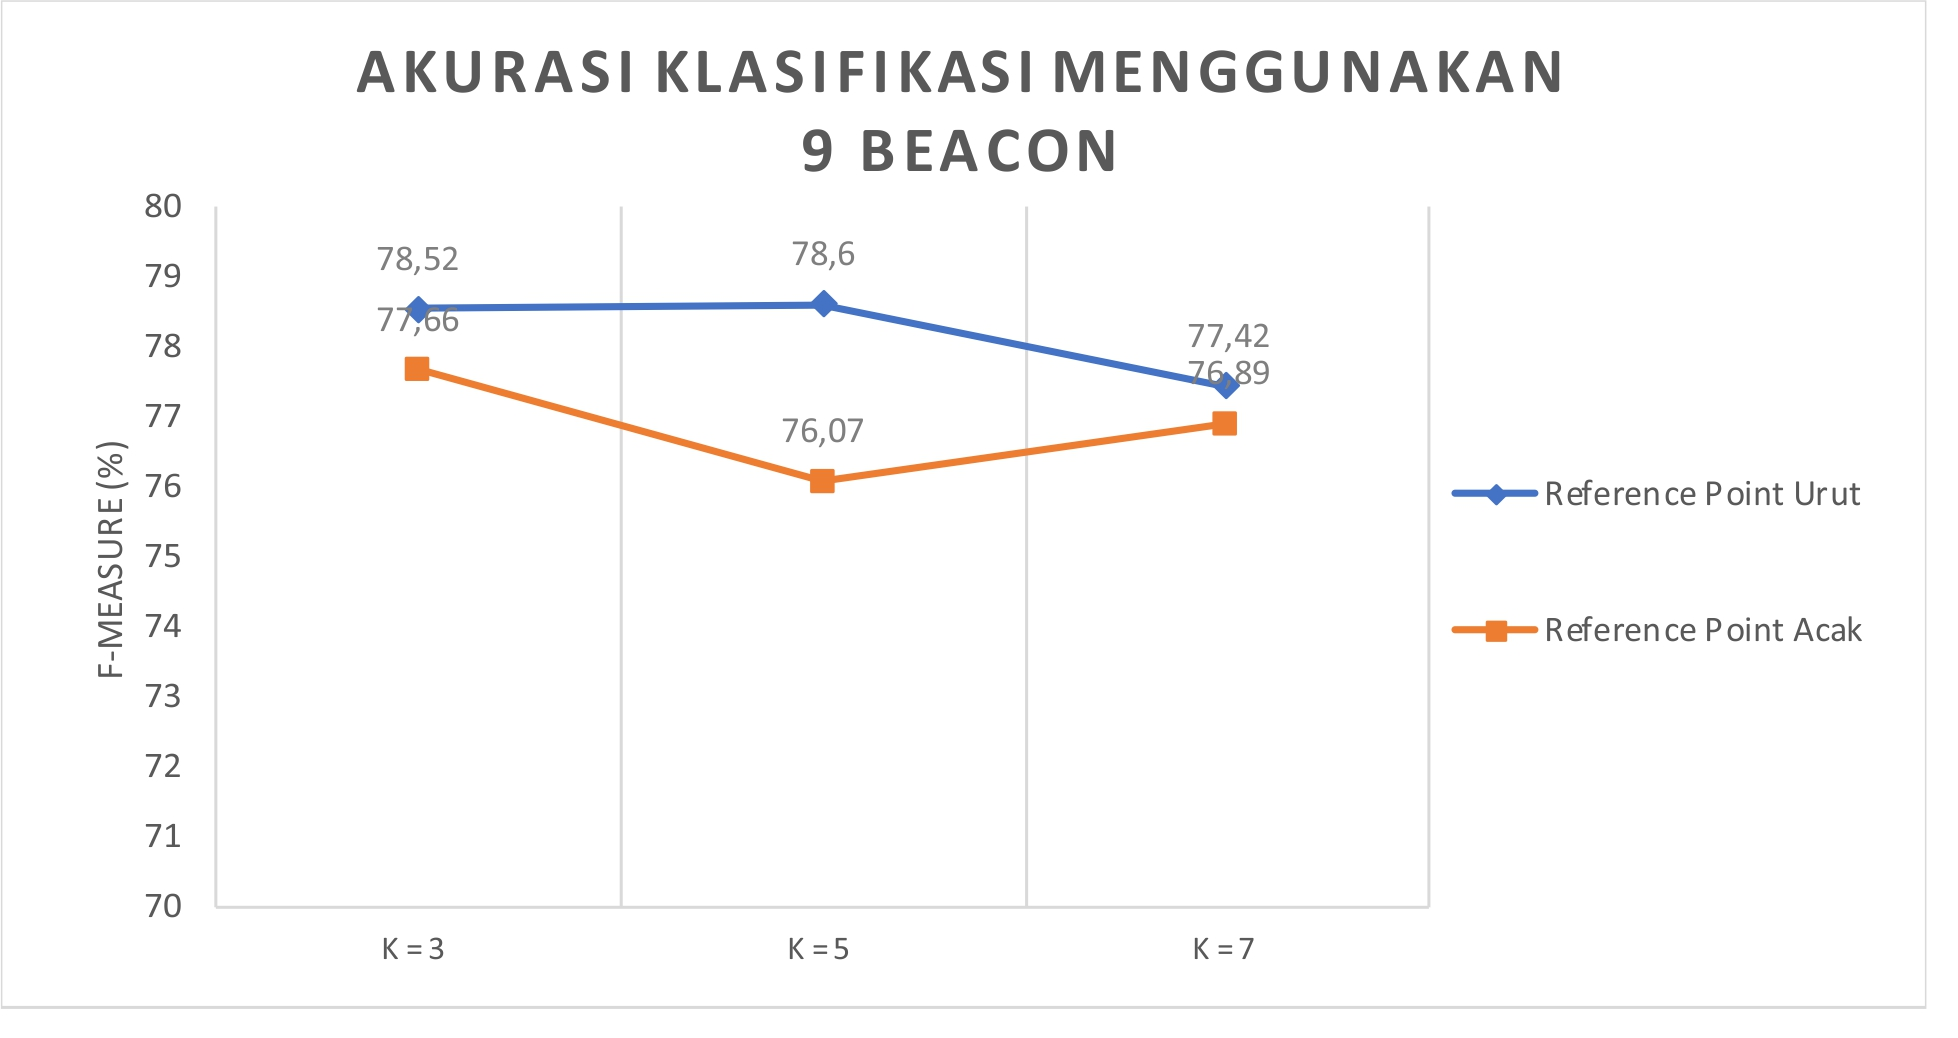
\includegraphics [width = 13cm, height= 7cm]{gambar/pengujian/grafik-akurasi-klasifikasi}}
		      \caption{Grafik Perbandingan F-Measure dengan Menggunakan Parameter Pengujian yang Berbeda.}
		      \label{gambar-grafik-akurasi-klasifikasi-9-beacon}
	      \end{figure}

	      \vspace{2cm}
	      \par Pengambilan data uji dilakukan untuk menguji tingkat keberhasilan klasifikasi dengan melihat akurasi tertinggi bergantung pada parameter nilai K yang digunakan. Pada pengujian ini terdapat titik yang sering salah diprediksi yaitu sebanyak 6 dari 6 kali pengujian. Lokasi titik yang sering salah diprediksi ditandai dengan lingkaran bewarna biru yang ditampilkan dalam bentuk ilustrasi denah yang dapat dilihat pada Gambar \ref{gambar-denah-titik-uji-b0302} dan Gambar \ref{gambar-denah-titik-uji-e0207}.
	      \vspace{0.2cm}
	      \begin{figure}[H]
		      \center
		      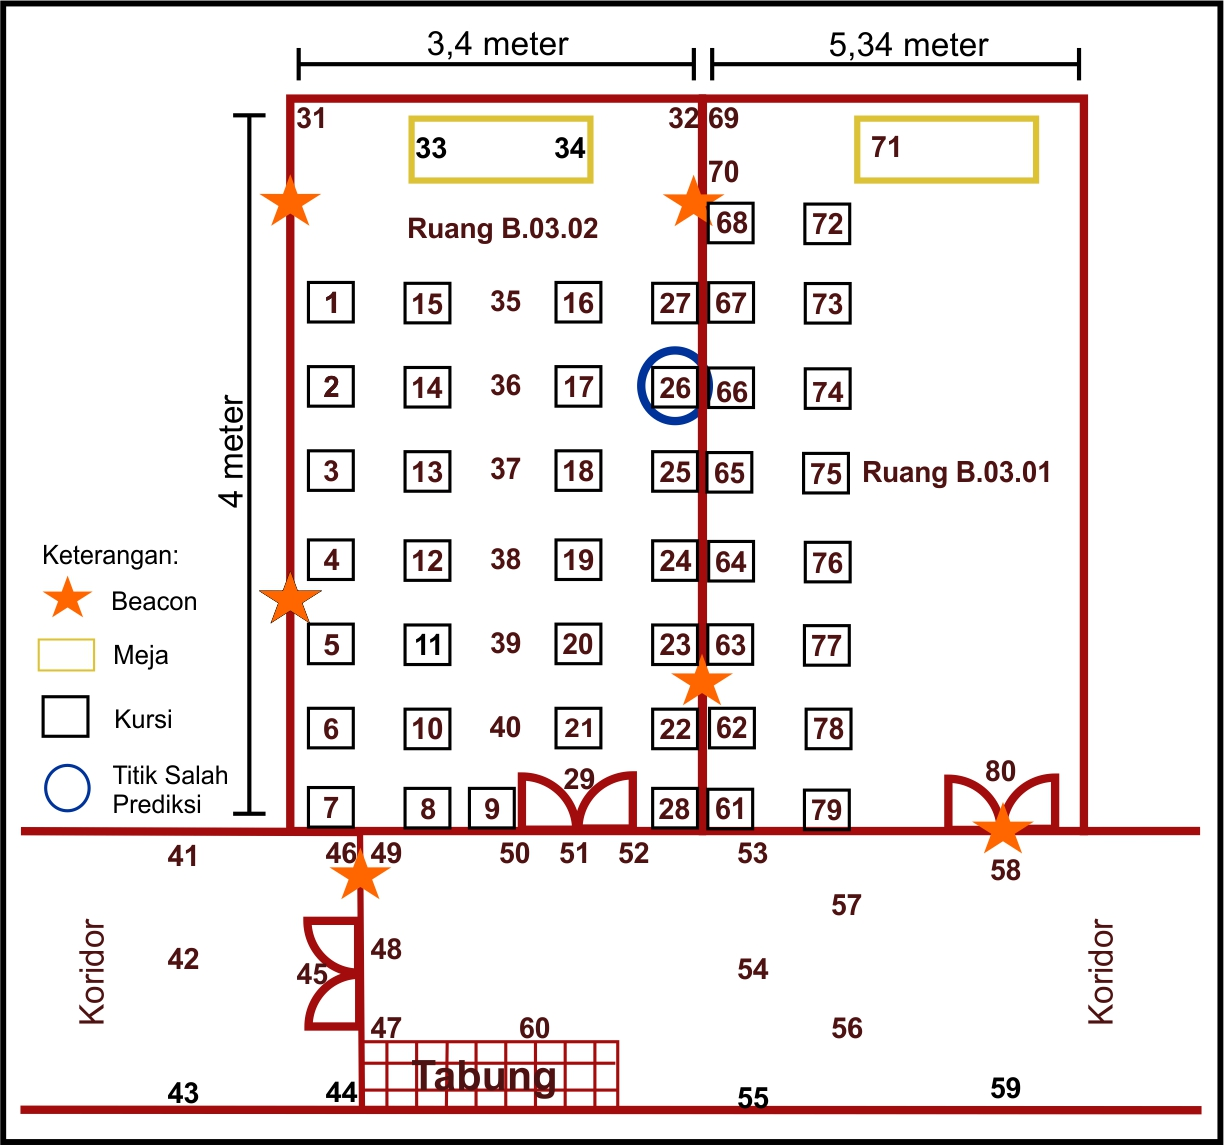
\includegraphics [width = 11cm, height= 9cm]{gambar/denah/B0302-Uji}
		      \caption{Lokasi Titik yang Sering Salah Diprediksi di Kelas B.03.02.}
		      \label{gambar-denah-titik-uji-b0302}
	      \end{figure}

	      \begin{figure}[H]
		      \center
		      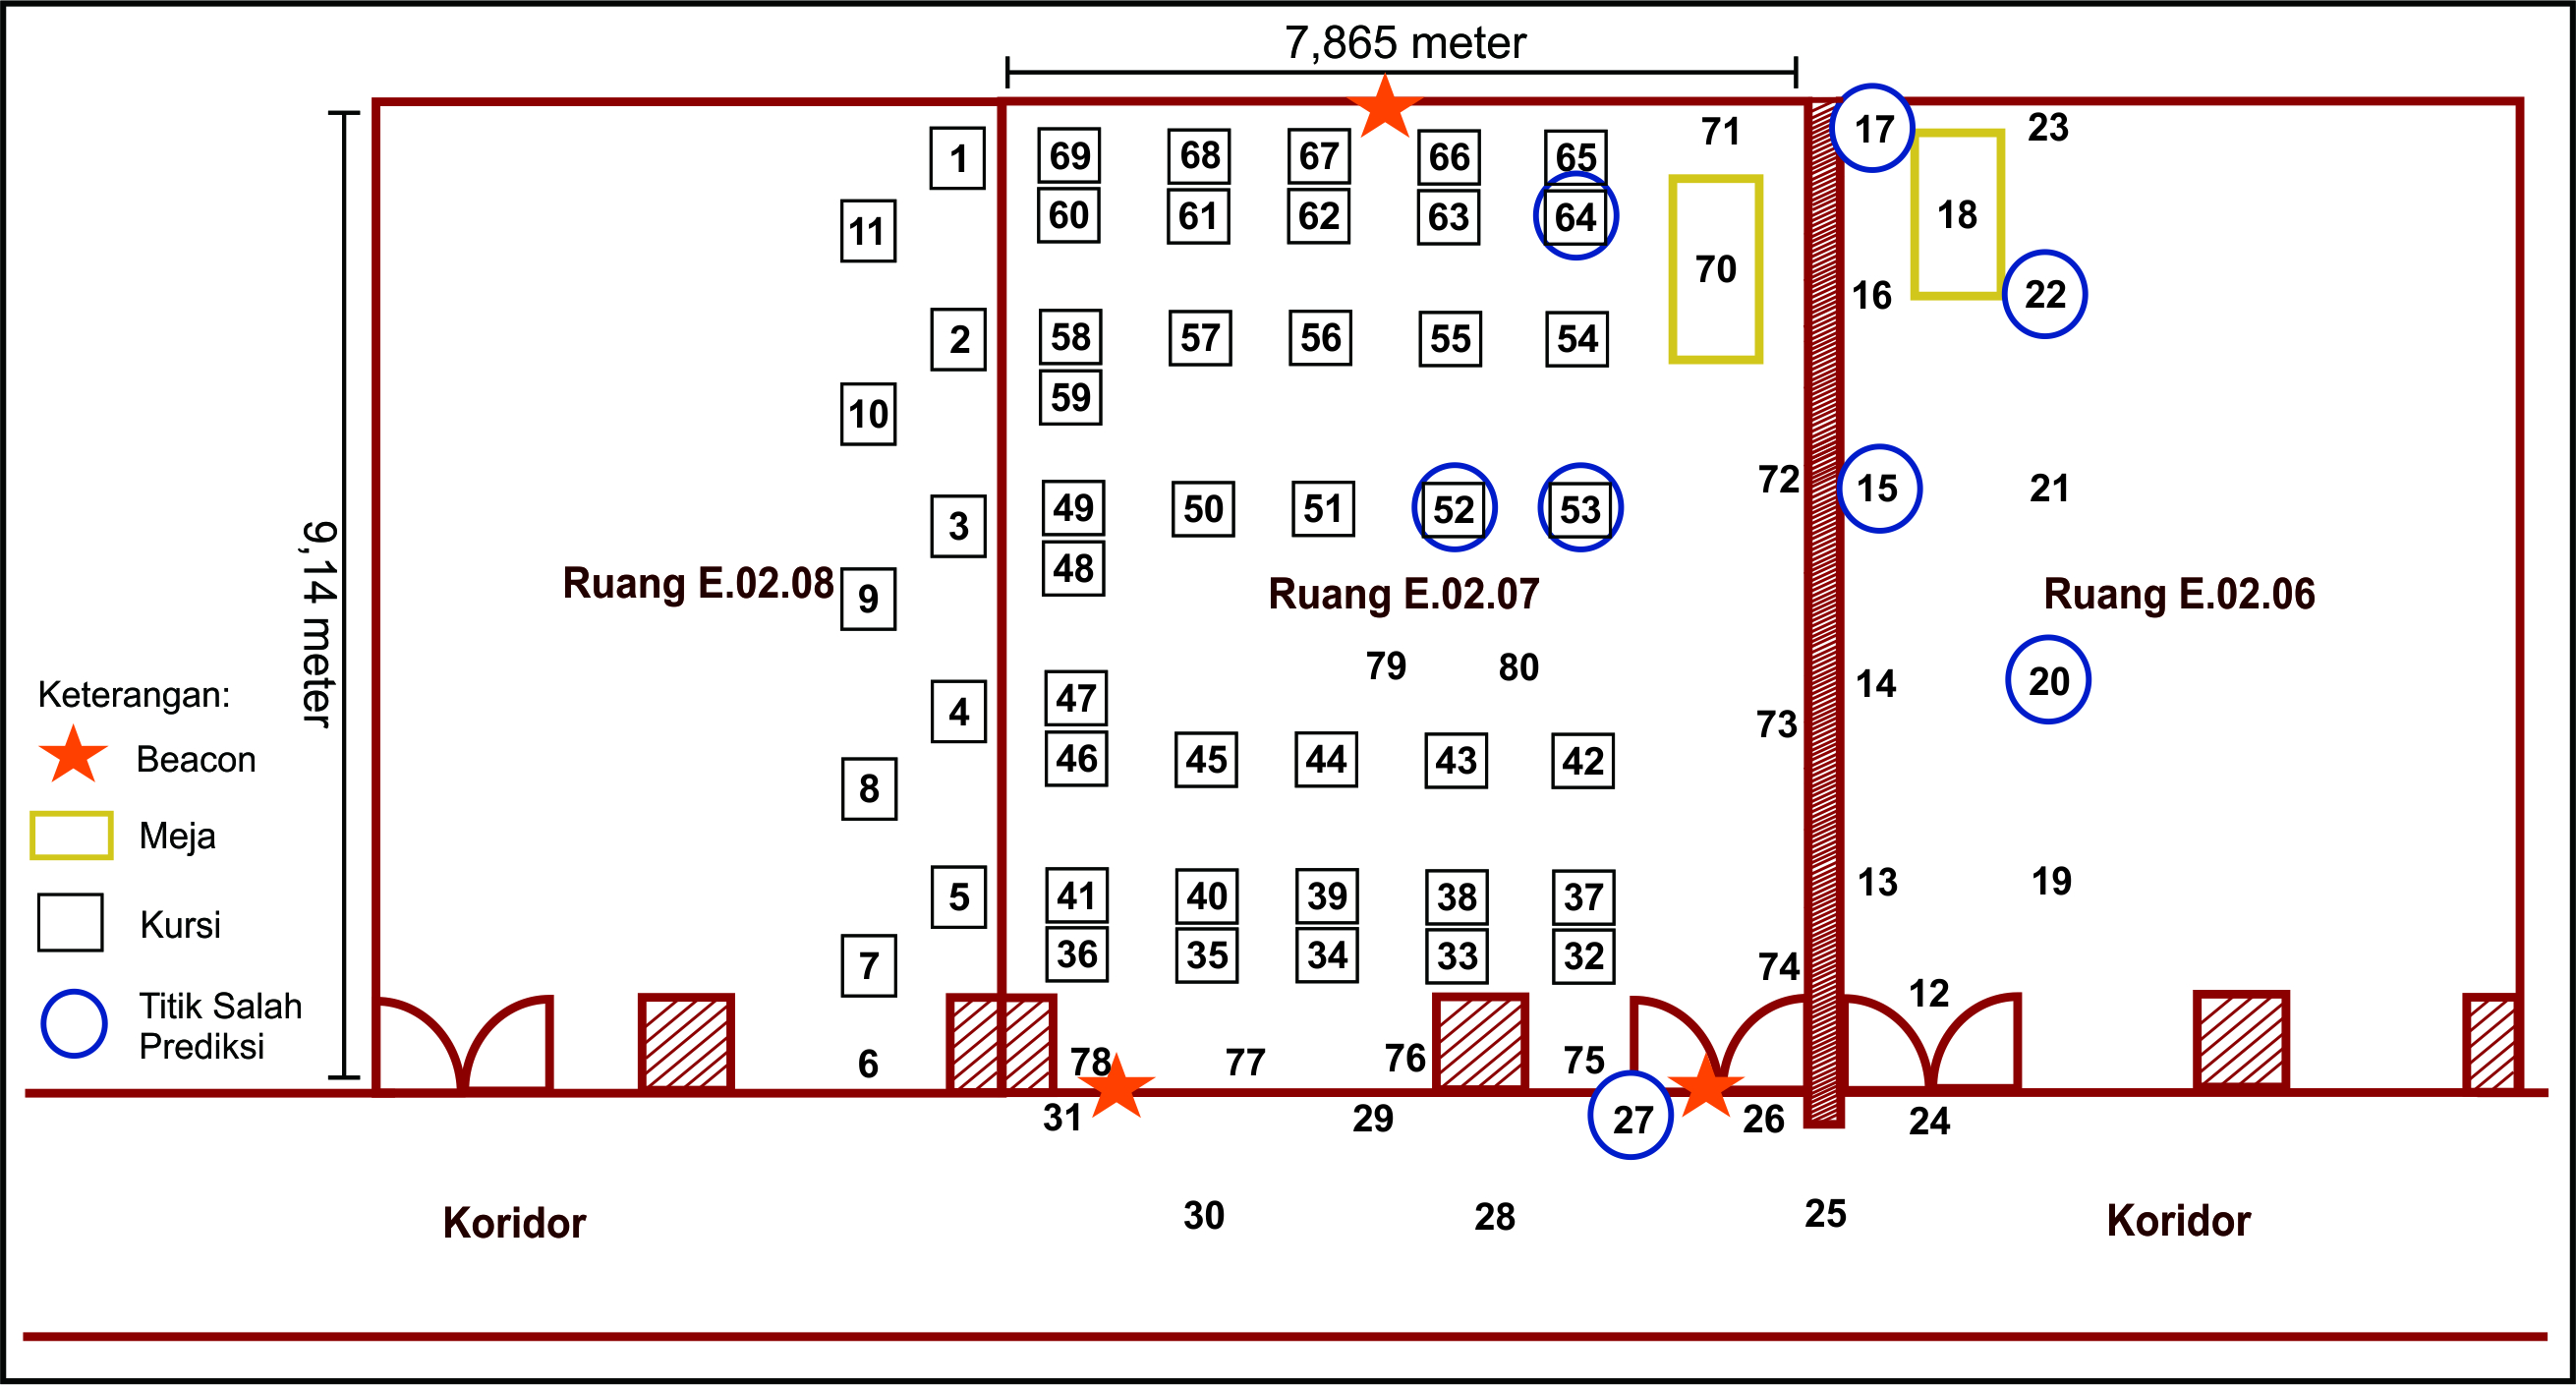
\includegraphics [width = 14cm, height= 8cm]{gambar/denah/E0207-Uji}
		      \caption{Lokasi Titik yang Sering Salah Diprediksi di Kelas E.02.07.}
		      \label{gambar-denah-titik-uji-e0207}
	      \end{figure}
	      %batas batas batas batas batas batas batas batas batas batas batas batas batas

	\item Pengujian Keakuratan Reference Point Berdasarkan Penggunaan Jumlah Beacon pada Ruang Kuliah B.03.02

	      \par Pengujian ini dianalisis menggunakan metode klasifikasi K-NN. Pengujian ini bertujuan untuk menganalisis tingkat keakuratan klasifikasi jenis \textit{reference point} terbaik yang digunakan dengan membandingkan penggunaan jumlah Beacon dengan melihat \textit{F-Measure} yang didapatkan dari setiap pengujian. Jumlah Beacon yang dibandingkan adalah 3 Beacon dan 6 Beacon. Data \textit{training} yang digunakan pada penelitian ini sebanyak 368 data kekuatan sinyal dengan masing-masing 120 data kekuatan sinyal untuk \textit{reference point} acak, 168 data kekuatan sinyal untuk \textit{reference point} urut dan 80 sebagai data uji. Pengumpulan data \textit{training} dilakukan dengan cara melakukan pemetaan kekuataan sinyal yang telah dijelaskan pada \textbf{BAB III}. Hasil dari proses pengujian metode klasifikasi K-NN menunjukkan bahwa dengan K=5 untuk data kekuatan sinyal \textit{reference point} acak menggunakan 6 Beacon, memiliki \textit{F-Measure} paling baik dengan nilai 96,20\% dibandingkan dengan parameter pengujian lainnya. Hasil pengujian menggunakan metode K-NN ini dapat dilihat secara detil pada Tabel \ref{tabelfmeasureee}.
	      % Please add the following required packages to your document preamble:
	      % \usepackage{multirow}
	      \begin{table}[H]
		      \fontsize{10}{12}\selectfont
		      \center
		      \caption{Perbandingan F-Measure}
		      \label{tabelfmeasureee}
		      \begin{tabular}{|c|c|l|c|c|c|}
			      \hline
			      Nilai K            & Jumlah BLE         & \multicolumn{1}{c|}{Jenis Titik} & Precision & Recall  & F-Measure \\ \hline
			      \multirow{2}{*}{3} & \multirow{2}{*}{3} & Urut                             & 67,24\%   & 97,50\% & 80,00\%   \\ \cline{3-6}
			                         &                    & Acak                             & 82,50\%   & 82,50\% & 82,50\%   \\ \hline
			      \multirow{2}{*}{5} & \multirow{2}{*}{3} & Urut                             & 67,24\%   & 97,50\% & 80,00\%   \\ \cline{3-6}
			                         &                    & Acak                             & 80,50\%   & 82,50\% & 81,50\%   \\ \hline
			      \multirow{2}{*}{7} & \multirow{2}{*}{3} & Urut                             & 67,24\%   & 97,50\% & 80,00\%   \\ \cline{3-6}
			                         &                    & Acak                             & 80,50\%   & 82,50\% & 81,50\%   \\ \hline
			      \multirow{2}{*}{3} & \multirow{2}{*}{6} & Urut                             & 90,70\%   & 97,50\% & 94,00\%   \\ \cline{3-6}
			                         &                    & Acak                             & 97,40\%   & 92,50\% & 95,00\%   \\ \hline
			      \multirow{2}{*}{5} & \multirow{2}{*}{6} & Urut                             & 90,70\%   & 97,50\% & 94,00\%   \\ \cline{3-6}
			                         &                    & Acak                             & 97,40\%   & 95,00\% & 96,20\%   \\ \hline
			      \multirow{2}{*}{7} & \multirow{2}{*}{6} & Urut                             & 90,70\%   & 97,50\% & 94,00\%   \\ \cline{3-6}
			                         &                    & Acak                             & 97,40\%   & 92,50\% & 95,00\%   \\ \hline
		      \end{tabular}
	      \end{table}

	      \par Ilustrasi dari perbandingan F-Measure setiap parameter pengujian ditampilkan pada Gambar \ref{gambar-grafik-akurasi-klasifikasi-6-beacon}.
	      \begin{figure}[H]
		      \center
		      \shadowbox
		      {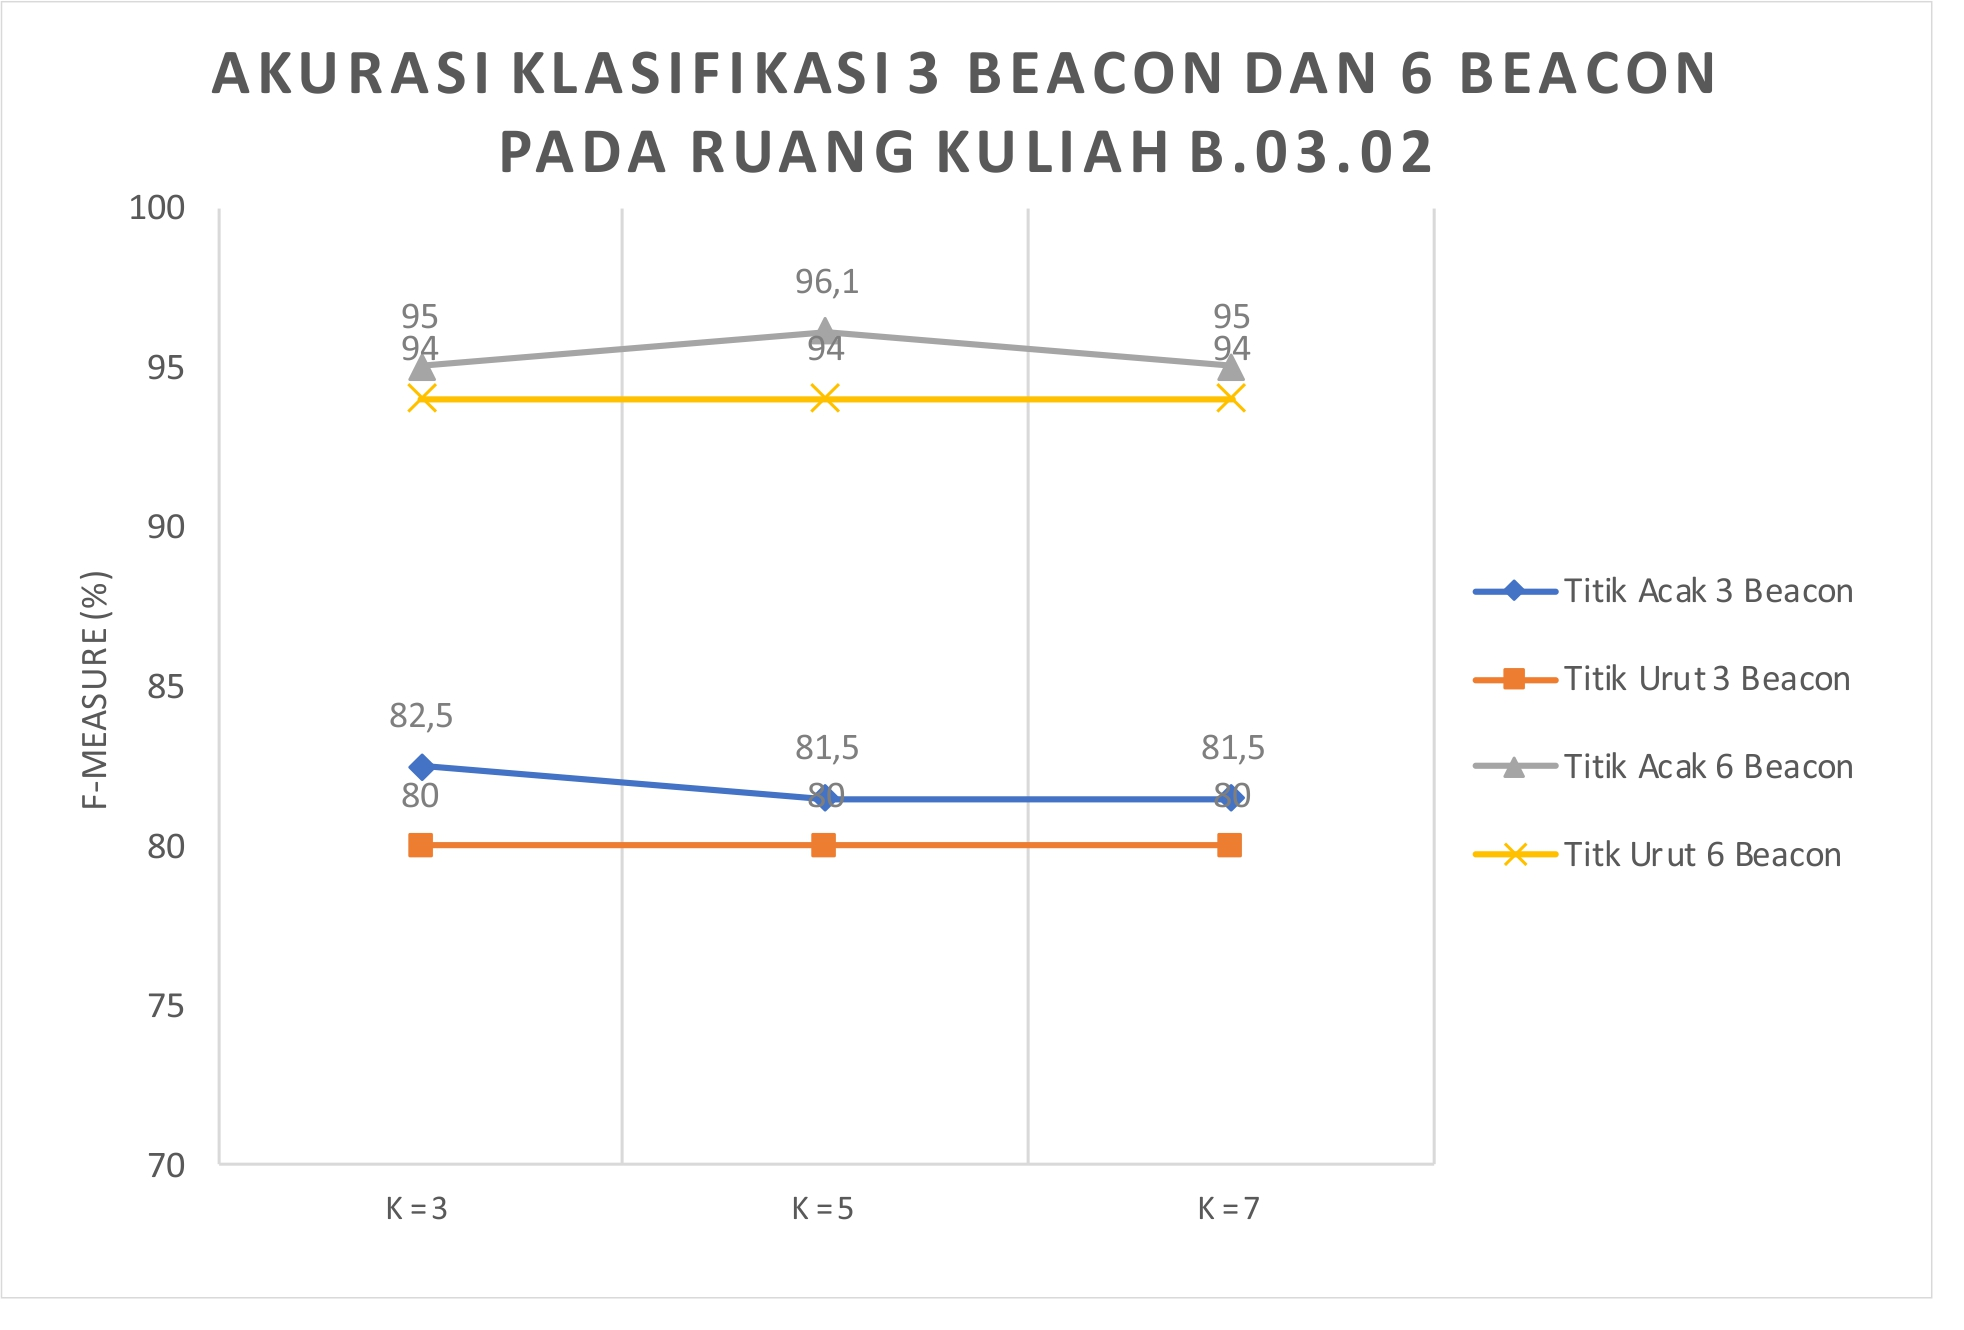
\includegraphics [width = 14cm, height= 8.7cm]{gambar/pengujian/grafik-akurasi-klasifikasi-kelas-b0302}}
		      \caption{Grafik Perbandingan F-Measure dengan Menggunakan Parameter Pengujian yang Berbeda.}
		      \label{gambar-grafik-akurasi-klasifikasi-6-beacon}
	      \end{figure}

	      \par Berdasarkan hasil pengujian dengan parameter nilai K yang berbeda menggunakan 3 Beacon dan 6 Beacon berdasarkan jenis \textit{reference point} yang digunakan, menunjukkan bahwa penggunaan 6 Beacon mengurangi kesalahan prediksi titik dibandingkan dengan 3 Beacon. Ilustrasi perbandingan tersebut dapat ditampilkan pada Gambar \ref{gambar-grafik-titik-salah-prediksi}.
	      \begin{figure}[H]
		      \center
		      \shadowbox
		      {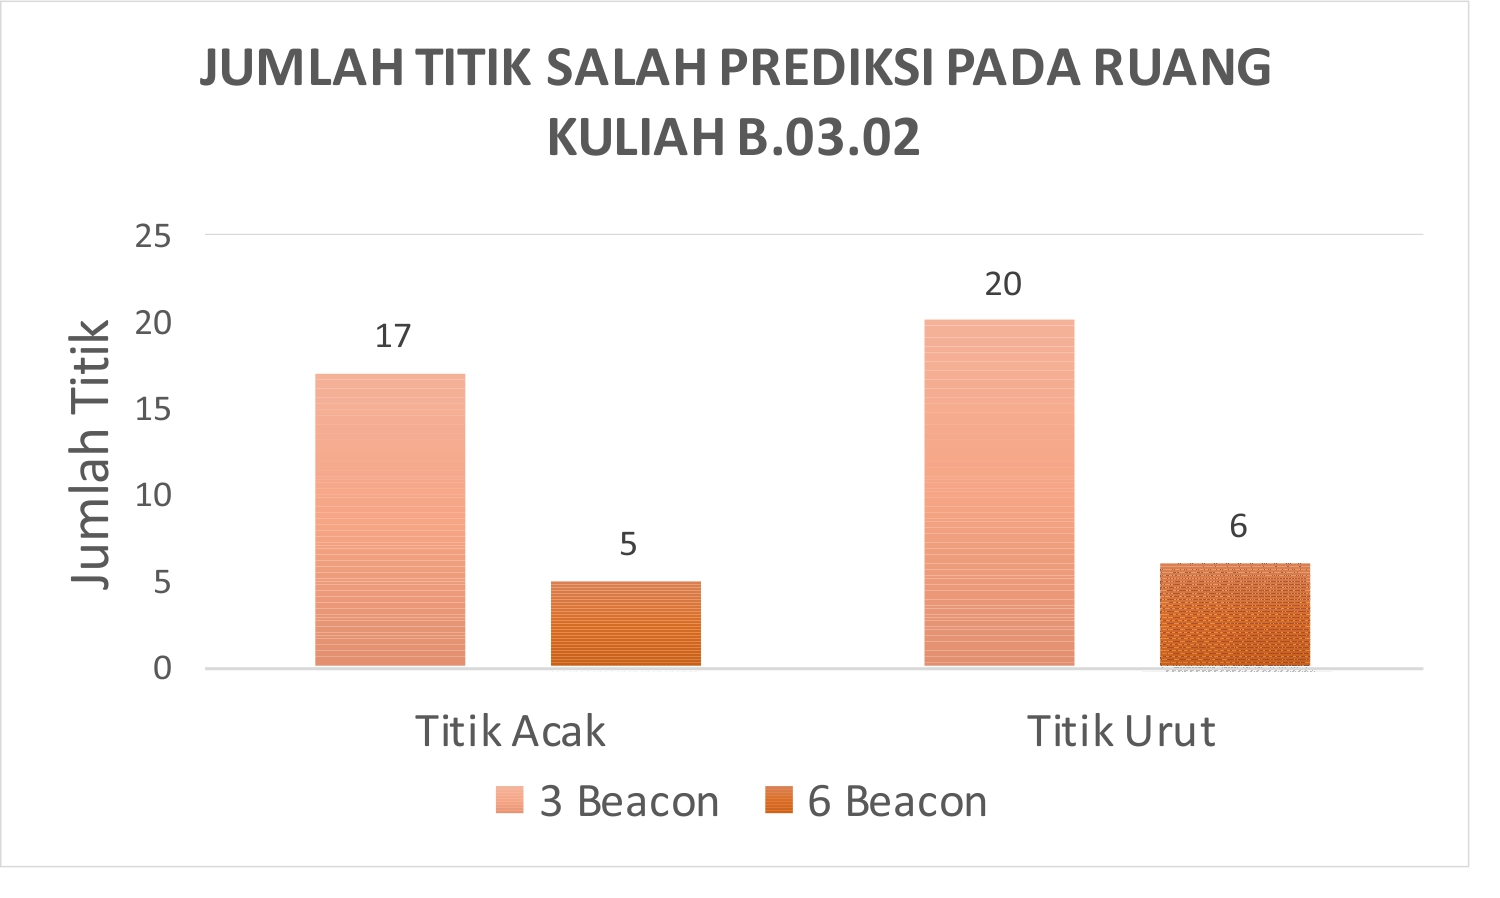
\includegraphics [width = 9cm, height= 5cm]{gambar/pengujian/grafik-titik-salah-prediksi}}
		      \caption{Grafik Jumlah Titik yang Salah Diprediksi.}
		      \label{gambar-grafik-titik-salah-prediksi}
	      \end{figure}


	      %batas batas batas batas batas batas batas batas batas batas batas batas batas	
\end{enumerate}

\subsection{Pengujian Usabilitas Menggunakan Metode UMUX}
\par Pengujian usabilitas bertujuan untuk menguji kelayakan dan kegunaan dari sistem yang akan digunakan oleh pengguna. Sebelum melakukan pengujian ini, adapun \textit{Test Plan} yang telah dibuat untuk yang dapat dilihat pada Tabel \ref{testplan-aplikasi-dosen}.

\begin{table}[H]
	\fontsize{10}{12}\selectfont
	\center
	\caption{\textit{Test Plan} Aplikasi SpecifyLocation}
	\label{testplan-aplikasi-dosen}
	\begin{tabular}{|l|l|l|l|l|}
		\hline
		\multicolumn{5}{|c|}{\textbf{Test Plan Aplikasi SpecifyLocation}}                                                                                                                                                                                                                                                                                                                                                              \\ \hline
		\multicolumn{5}{|l|}{\begin{tabular}[c]{@{}l@{}}Lokasi:\\ Lantai 1 Gedung A FMIPA USK \\Lantai 3 Gedung A FMIPA USK\end{tabular}}                                                                                                                                                                                                                                                                                              \\ \hline
		\multicolumn{5}{|l|}{\begin{tabular}[c]{@{}l@{}}Skenario:\\ 1. Pengguna membuka aplikasi.\\ 2. Pengguna memahami tampilan halaman awal. \\ 3. Pengguna menekan cek lokasi di lantai 1 gedung a FMIPA USK. \\ 4. Pengguna menekan cek lokasi di lantai 3 gedung a FMIPA USK.\\ 5. Pengguna melihat hasil prediksi lokasi yang dilakukan oleh aplikasi.\\6. Pengguna melihat estimasi jumlah orang di dalam gedung\end{tabular}} \\ \hline
		\multicolumn{5}{|l|}{\begin{tabular}[c]{@{}l@{}}Alat:\\ 1. Smartphone Android\\ 2. Beacon\end{tabular}}                                                                                                                                                                                                                                                                                                                        \\ \hline
		\multicolumn{5}{|l|}{\begin{tabular}[c]{@{}l@{}}Hasil:\\ Hasil pengujian dapat dilihat pada tabel dan lampiran.\end{tabular}}                                                                                                                                                                                                                                                                                                  \\ \hline
	\end{tabular}
\end{table}

\par Pengujian dengan menggunakan metode UMUX dilakukan dengan memberikan kuisioner kepada responden. Kuisioner tersebut berisi 4 pertanyaan seperti yang sudah dibahas pada \textbf{BAB III}. Pengujian ini memiliki [Jumlah responden] responden. Hasil skor pengujian metode UMUX yang dilakukan dapat dilihat pada tabel \ref{sus-aplikasi-dosen} berikut.
% \par Pengujian dengan metode SUS dilakukan dengan memberikan kuisioner kepada responden. Kuisioner tersebut berisi 10 pertanyaan seperti yang telah dibahas pada. Pengujian Aplikasi Kehadiran Dosen memiliki responden berjumlah 5 orang sedangkan pengujian Aplikasi Kehadiran Mahasiswa memiliki responden berjumlah 9 orang. Hasil skor pengujian metode SUS yang dilakukan dapat dilihat pada Tabel \ref{sus-aplikasi-dosen} dan Tabel \ref{sus-aplikasi-mahasiswa} berikut.
%TABEL SUS APLIKASI DOSEN%
\begin{table}[H]
	\fontsize{10}{12}\selectfont
	\center
	\caption{Hasil Pengujian SUS Aplikasi Kehadiran Dosen}
	\label{sus-aplikasi-dosen}
	\begin{tabular}{|c|c|c|c|c|c|c|c|c|c|c|c|}
		\hline
		\multirow{2}{*}{\textbf{Responden}}         & \multicolumn{10}{c|}{\textbf{Kode Pertanyaan}} & \multirow{2}{*}{\textbf{Skor SUS}}                                                                                                                                              \\ \cline{2-11}
		                                            & \textbf{R1}                                    & \textbf{R2}                        & \textbf{R3} & \textbf{R4} & \textbf{R5} & \textbf{R6} & \textbf{R7} & \textbf{R8} & \textbf{R9} & \multicolumn{1}{l|}{\textbf{R10}} &      \\ \hline
		1                                           & 3                                              & 2                                  & 4           & 1           & 4           & 4           & 4           & 3           & 4           & 2                                 & 67,5 \\ \hline
		2                                           & 5                                              & 2                                  & 5           & 4           & 4           & 2           & 4           & 2           & 4           & 5                                 & 67,5 \\ \hline
		3                                           & 4                                              & 2                                  & 4           & 1           & 4           & 2           & 4           & 1           & 4           & 4                                 & 75,0 \\ \hline
		4                                           & 5                                              & 1                                  & 5           & 2           & 5           & 2           & 5           & 1           & 5           & 1                                 & 95,0 \\ \hline
		5                                           & 5                                              & 2                                  & 5           & 1           & 4           & 2           & 5           & 2           & 5           & 2                                 & 87,5 \\ \hline
		\multicolumn{11}{|c|}{\textbf{Rata - Rata}} & \textbf{78,5}                                                                                                                                                                                                                    \\ \hline
	\end{tabular}
\end{table}

\par Berdasarkan hasil pengujian dengan menggunakan metode UMUX yang telah dilakukan diatas, hasil rata-rata pengujian Aplikasi SpecifyLocation mendapatkan skor sebesar 78,5\% . Dapat dilihat bahwa aplikasi yang telah dibangun ini memiliki skor interpretasi \textbf{"dapat diterima"} berdasarkan Tabel 3.4.

\subsection{Pengujian Fungsionalitas Menggunakan Blackbox}
\par Pengujian \textit{Blackbox} dilakukan dengan tujuan untuk menguji fungsionalitas dari aplikasi dengan menjalankan aplikasi tersebut apakah sesuai dengan alur bisnis yang diinginkan. Pengujian ini melihat fungsi yang tidak sesuai pada aplikasi dan kesalahan-kesalahan aplikasi dalam mengerjakan suatu perintah. Pengujian ini dilakukan pada Aplikasi Mapping, Aplikasi Kehadiran Dosen, Aplikasi Kehadiran Mahasiswa, dan Aplikasi Web Rekap Kehadiran Dosen dan Mahasiswa. Beberapa fitur aplikasi yang diuji menggunakan \textit{Blackbox Testing} dapat dilihat pada Tabel \ref{blackbox-aplikasi-mapping}, Tabel \ref{blackbox-aplikasi-dosen}, Tabel \ref{blackbox-aplikasi-mahasiswa}, dan Tabel \ref{blackbox-web-admin}.
%TABEL APLIKASI MAPPING%
\begin{table}[H]
	\fontsize{10}{12}\selectfont
	\center
	\caption{Pengujian \textit{Blackbox} Aplikasi Mapping}
	\label{blackbox-aplikasi-mapping}
	\begin{tabular}{|c|l|l|l|c|}
		\hline
		\textbf{No.} & \multicolumn{1}{c|}{\textbf{Nama Pengujian}}                                       & \multicolumn{1}{c|}{\textbf{Skenario}}                                                                                               & \multicolumn{1}{c|}{\textbf{Tampilan}}                                                                    & \textbf{Hasil}                \\ \hline
		1.           & \begin{tabular}[c]{@{}l@{}}Menghidupkan \\ Bluetooth\end{tabular}                  & \begin{tabular}[c]{@{}l@{}}Klik tombol \textbf{Allow} \\ pada notifikasi yang\\ muncul\end{tabular}                                  & \begin{tabular}[c]{@{}l@{}}Bluetooth akan \\ hidup\end{tabular}                                           & Berhasil                      \\ \hline
		2.           & \begin{tabular}[c]{@{}l@{}}Lakukan proses \\ pemindaian \\ sinyal BLE\end{tabular} & Klik tombol \textbf{"Scan"}                                                                                                          & \begin{tabular}[c]{@{}l@{}}Muncul nama BLE, \\ MAC Address BLE \\ dan kekuatan sinyal \\ BLE\end{tabular} & Berhasil                      \\ \hline
		3.           & \begin{tabular}[c]{@{}l@{}}Menyimpan data \\ ke tabel titik acak\end{tabular}      & \begin{tabular}[c]{@{}l@{}}Mengisi nama ruang \\ kemudian klik tombol \\ \textbf{Save to} dan pilih \\ tabel titik acak\end{tabular} & \begin{tabular}[c]{@{}l@{}}Muncul \textit{pop up} \\ untuk memilih \\ tabel\end{tabular}                  & Berhasil                      \\ \hline
		4.           & \begin{tabular}[c]{@{}l@{}}Menyimpan data \\ ke tabel titik urut\end{tabular}      & \begin{tabular}[c]{@{}l@{}}Mengisi nama ruang \\ kemudian klik tombol \\ \textbf{Save to} dan pilih \\ tabel titik urut\end{tabular} & \begin{tabular}[c]{@{}l@{}}Muncul \textit{pop up} \\ untuk memilih \\ tabel\end{tabular}                  & Berhasil                      \\ \hline
		5.           & \begin{tabular}[c]{@{}l@{}}Melihat data \\ yang tersimpan\end{tabular}             & \begin{tabular}[c]{@{}l@{}}Klik tombol \\ \textbf{Show Data}\end{tabular}                                                            & \begin{tabular}[c]{@{}l@{}}Diarahkan ke \\ halaman daftar \\ data yang tersimpan\end{tabular}             & Berhasil                      \\ \hline
		6.           & \begin{tabular}[c]{@{}l@{}}Menghapus data \\ yang tersimpan\end{tabular}           & \begin{tabular}[c]{@{}l@{}}Klik icon \textbf{Tong} \\ \textbf{Sampah}\end{tabular}                                                   & \begin{tabular}[c]{@{}l@{}}Muncul notifikasi \\ dan konfirmasi \\ untuk menghapus \\ data\end{tabular}    & \multicolumn{1}{l|}{Berhasil} \\ \hline
	\end{tabular}
\end{table}

%BLACKBOX APLIKASI DOSEN%
\begin{table}[H]
	\fontsize{10}{12}\selectfont
	\center
	\caption{Pengujian \textit{Blackbox } Aplikasi Kehadiran Dosen}
	\label{blackbox-aplikasi-dosen}
	\begin{tabular}{|c|l|l|l|c|}
		\hline
		No. & \multicolumn{1}{c|}{\textbf{Nama Pengujian}}                                                                     & \multicolumn{1}{c|}{\textbf{Skenario}}                                                                                    & \multicolumn{1}{c|}{\textbf{Tampilan}}                                                                                          & Hasil    \\ \hline
		1.  & \begin{tabular}[c]{@{}l@{}}Melakukan \textit{log in} \\ ke aplikasi\end{tabular}                                 & \begin{tabular}[c]{@{}l@{}}Klik tombol \textbf{Submit} \\ setelah selesai \\ mengisi form \textit{log in}\end{tabular}    & \begin{tabular}[c]{@{}l@{}}Diarahkan ke \\ halaman beranda \\ aplikasi apabila \\ berhasil \textit{log in}\end{tabular}         & Berhasil \\ \hline
		2.  & \begin{tabular}[c]{@{}l@{}}Melihat informasi \\ suatu mata kuliah\end{tabular}                                   & \begin{tabular}[c]{@{}l@{}}Klik salah satu daftar \\ mata kuliah\end{tabular}                                             & \begin{tabular}[c]{@{}l@{}}Diarahkan ke \\ halaman informasi \\ mata kuliah\end{tabular}                                        & Berhasil \\ \hline
		3.  & \begin{tabular}[c]{@{}l@{}}Menghidupkan \\ Bluetooth\end{tabular}                                                & \begin{tabular}[c]{@{}l@{}}Klik tombol \textbf{Allow} \\ pada notifikasi yang \\ muncul\end{tabular}                      & \begin{tabular}[c]{@{}l@{}}Bluetooth akan \\ menyala\end{tabular}                                                               & Berhasil \\ \hline
		4.  & \begin{tabular}[c]{@{}l@{}}Melihat daftar \\ nama mahasiswa \\ yang mengambil  \\ suatu mata kuliah\end{tabular} & \begin{tabular}[c]{@{}l@{}}Klik tombol \\ \textbf{Show Students} pada \\ halaman informasi \\ mata kuliah\end{tabular}    & \begin{tabular}[c]{@{}l@{}}Diarahkan ke \\ halaman daftar \\ nama mahasiswa\end{tabular}                                        & Berhasil \\ \hline
		5.  & \begin{tabular}[c]{@{}l@{}}Memulai proses \\ kehadiran\end{tabular}                                              & \begin{tabular}[c]{@{}l@{}}Klik tombol \\ \textbf{Start Attendance} \\ pada halaman \\ informasi mata kuliah\end{tabular} & \begin{tabular}[c]{@{}l@{}}Secara \textit{background} \\ \textit{proccess} aplikasi \\ akan memproses \\ kehadiran\end{tabular} & Berhasil \\ \hline
	\end{tabular}
\end{table}

%BLACKBOX APLIKASI MAHASISWA%
\begin{table}[H]
	\fontsize{10}{12}\selectfont
	\center
	\caption{Pengujian \textit{Blackbox} Aplikasi Kehadiran Mahasiswa}
	\label{blackbox-aplikasi-mahasiswa}
	\begin{tabular}{|c|l|l|l|c|}
		\hline
		No. & \multicolumn{1}{c|}{\textbf{Nama Pengujian}}                                          & \multicolumn{1}{c|}{\textbf{Skenario}}                                                                                    & \multicolumn{1}{c|}{\textbf{Tampilan}}                                                                                          & Hasil                         \\ \hline
		1.  & \begin{tabular}[c]{@{}l@{}}Melakukan \textit{log in}\\ ke aplikasi\end{tabular}       & \begin{tabular}[c]{@{}l@{}}Klik tombol \textbf{Submit} \\ setelah selesai \\ mengisi form \textit{log in}\end{tabular}    & \begin{tabular}[c]{@{}l@{}}Diarahkan ke \\ halaman beranda \\ aplikasi apabila \\ berhasil \textit{log in}\end{tabular}         & Berhasil                      \\ \hline
		2.  & \begin{tabular}[c]{@{}l@{}}Melihat daftar \\ mata kuliah \\ yang diambil\end{tabular} & Klik icon \textbf{My Course}                                                                                              & \begin{tabular}[c]{@{}l@{}}Diarahkan ke \\ halaman daftar \\ mata kuliah\end{tabular}                                           & Berhasil                      \\ \hline
		3.  & \begin{tabular}[c]{@{}l@{}}Melihat profil \\ data diri\end{tabular}                   & Klik icon \textbf{My Profile                                                                                            } & \begin{tabular}[c]{@{}l@{}}Diarahkan ke \\ halaman profil\end{tabular}                                                          & \multicolumn{1}{l|}{Berhasil} \\ \hline
		4.  & \begin{tabular}[c]{@{}l@{}}Menghidupkan \\ Bluetooth\end{tabular}                     & \begin{tabular}[c]{@{}l@{}}Klik tombol \textbf{Allow} \\ pada notifikasi \\ yang muncul\end{tabular}                      & \begin{tabular}[c]{@{}l@{}}Bluetooth akan \\ menyala\end{tabular}                                                               & Berhasil                      \\ \hline
		5.  & \begin{tabular}[c]{@{}l@{}}Memulai \\ proses kehadiran\end{tabular}                   & \begin{tabular}[c]{@{}l@{}}Klik tombol \\ \textbf{Start Attendance} \\ pada salah satu \\ daftar mata kuliah\end{tabular} & \begin{tabular}[c]{@{}l@{}}Secara \textit{background} \\ \textit{proccess} aplikasi \\ akan memproses \\ kehadiran\end{tabular} & Berhasil                      \\ \hline
	\end{tabular}
\end{table}

%BLACKBOX WEB ADMIN%
\begin{table}[H]
	\fontsize{10}{12}\selectfont
	\center
	\caption{Pengujian \textit{Blackbox} Aplikasi Web Rekap Kehadiran Dosen dan Mahasiswa}
	\label{blackbox-web-admin}
	\begin{tabular}{|c|l|l|l|c|}
		\hline
		No. & \multicolumn{1}{c|}{\textbf{Nama Pengujian}}                                          & \multicolumn{1}{c|}{\textbf{Skenario}}                                                                                    & \multicolumn{1}{c|}{\textbf{Tampilan}}                                                                                          & Hasil                         \\ \hline
		1.  & \begin{tabular}[c]{@{}l@{}}Melakukan \textit{log in}\\ ke aplikasi\end{tabular}       & \begin{tabular}[c]{@{}l@{}}Klik tombol \\ \textbf{Submit} setelah \\ selesai mengisi \\ form \textit{log in}\end{tabular} & \begin{tabular}[c]{@{}l@{}}Diarahkan ke \\ halaman beranda \\ aplikasi apabila \\ berhasil \textit{log in}\end{tabular}         & Berhasil                      \\ \hline
		2.  & \begin{tabular}[c]{@{}l@{}}Melihat daftar \\ mata kuliah \\ yang diambil\end{tabular} & \begin{tabular}[c]{@{}l@{}}Klik icon \\ \textbf{My Course}\end{tabular}                                                   & \begin{tabular}[c]{@{}l@{}}Diarahkan ke \\ halaman daftar \\ mata kuliah\end{tabular}                                           & Berhasil                      \\ \hline
		3.  & \begin{tabular}[c]{@{}l@{}}Melihat profil \\ data diri\end{tabular}                   & \begin{tabular}[c]{@{}l@{}}Klik icon \\ \textbf{My Profile}\end{tabular}                                                  & \begin{tabular}[c]{@{}l@{}}Diarahkan ke \\ halaman profil\end{tabular}                                                          & \multicolumn{1}{l|}{Berhasil} \\ \hline
		4.  & \begin{tabular}[c]{@{}l@{}}Menghidupkan \\ Bluetooth\end{tabular}                     & \begin{tabular}[c]{@{}l@{}}Klik tombol \\ \textbf{Allow} pada \\ notifikasi yang\\ muncul\end{tabular}                    & \begin{tabular}[c]{@{}l@{}}Bluetooth akan \\ menyala\end{tabular}                                                               & Berhasil                      \\ \hline
		5.  & \begin{tabular}[c]{@{}l@{}}Memulai \\ proses kehadiran\end{tabular}                   & \begin{tabular}[c]{@{}l@{}}Klik tombol \\ \textbf{Start Attendance} \\ pada salah satu \\ daftar mata kuliah\end{tabular} & \begin{tabular}[c]{@{}l@{}}Secara \textit{background} \\ \textit{proccess} aplikasi \\ akan memproses \\ kehadiran\end{tabular} & Berhasil                      \\ \hline
	\end{tabular}
\end{table}

%AKHIR DARI TABEL%
\par Berdasarkan hasil \textit{Blackbox Testing} dari tabel diatas menunjukkan bahwa Aplikasi Mapping, Aplikasi Kehadiran Dosen, Aplikasi Kehadiran Mahasiswa, dan Aplikasi Web Rekap Kehadiran Dosen dan Mahasiswa dapat berjalan dengan baik dibuktikan dengan  \textbf{"berhasil"} pada kolom hasil pengujian masing-masing fitur yang dikerjakan.


\begin{comment}
\bibliography{daftar-pustaka}
\end{comment}